\documentclass[a4paper,12pt, oneside]{book}

% \usepackage{fullpage}
\usepackage[italian]{babel}
\usepackage[utf8]{inputenc}
\usepackage{amssymb}
\usepackage{amsthm}
\usepackage{graphics}
\usepackage{amsfonts}
\usepackage{listings}
\usepackage{amsmath}
\usepackage{amstext}
\usepackage{engrec}
\usepackage{rotating}
\usepackage{verbatim}
\usepackage[safe,extra]{tipa}
%\usepackage{showkeys}
\usepackage{multirow}
\usepackage{hyperref}
\usepackage{microtype}
\usepackage{fontspec}
\usepackage{enumerate}
\usepackage{physics}
\usepackage{braket}
\usepackage{marginnote}
\usepackage{pgfplots}
\usepackage{cancel}
\usepackage{polynom}
\usepackage{booktabs}
\usepackage{enumitem}
\usepackage{framed}
\usepackage{pdfpages}
\usepackage{pgfplots}
\usepackage{algorithm}
% \usepackage{algpseudocode}
\usepackage[cache=false]{minted}
\usepackage{mathtools}
\usepackage[noend]{algpseudocode}

\usepackage{tikz}\usetikzlibrary{er}\tikzset{multi  attribute /.style={attribute
    ,double  distance =1.5pt}}\tikzset{derived  attribute /.style={attribute
    ,dashed}}\tikzset{total /.style={double  distance =1.5pt}}\tikzset{every
  entity /.style={draw=orange , fill=orange!20}}\tikzset{every  attribute
  /.style={draw=MediumPurple1, fill=MediumPurple1!20}}\tikzset{every
  relationship /.style={draw=Chartreuse2,
    fill=Chartreuse2!20}}\newcommand{\key}[1]{\underline{#1}}
  \usetikzlibrary{arrows.meta}
  \usetikzlibrary{decorations.markings}
  \usetikzlibrary{arrows,shapes,backgrounds,petri}
\tikzset{
  place/.style={
        circle,
        thick,
        draw=black,
        minimum size=6mm,
    },
  transition/.style={
    rectangle,
    thick,
    fill=black,
    minimum width=8mm,
    inner ysep=2pt
  },
  transitionv/.style={
    rectangle,
    thick,
    fill=black,
    minimum height=8mm,
    inner xsep=2pt
    }
  } 
\usetikzlibrary{automata,positioning,chains,fit,shapes}
\usepackage{fancyhdr}
\pagestyle{fancy}
\fancyhead[LE,RO]{\slshape \rightmark}
\fancyhead[LO,RE]{\slshape \leftmark}
\fancyfoot[C]{\thepage}
\usepackage[usenames,dvipsnames]{pstricks}
\usepackage{epsfig}
\usepackage{pst-grad} % For gradients
\usepackage{pst-plot} % For axes
\usepackage[space]{grffile} % For spaces in paths
\usepackage{etoolbox} % For spaces in paths
\makeatletter % For spaces in paths
\patchcmd\Gread@eps{\@inputcheck#1 }{\@inputcheck"#1"\relax}{}{}
\makeatother

\title{Teoria dell'Informazione e Crittografia}
\author{UniShare\\\\Davide Cozzi\\\href{https://t.me/dlcgold}{@dlcgold}}
\date{}

\pgfplotsset{compat=1.13}
\begin{document}
\maketitle

\definecolor{shadecolor}{gray}{0.80}
\setlist{leftmargin = 2cm}
\newtheorem{teorema}{Teorema}
\newtheorem{definizione}{Definizione}
\newtheorem{esempio}{Esempio}
\newtheorem{corollario}{Corollario}
\newtheorem{lemma}{Lemma}
\newtheorem{osservazione}{Osservazione}
\newtheorem{nota}{Nota}
\newtheorem{esercizio}{Esercizio}
\algdef{SE}[DOWHILE]{Do}{doWhile}{\algorithmicdo}[1]{\algorithmicwhile\ #1}
\tableofcontents
\renewcommand{\chaptermark}[1]{%
  \markboth{\chaptername
    \ \thechapter.\ #1}{}}
\renewcommand{\sectionmark}[1]{\markright{\thesection.\ #1}}
\newcommand{\floor}[1]{\lfloor #1 \rfloor}
\newcommand{\MYhref}[3][blue]{\href{#2}{\color{#1}{#3}}}%
\chapter{Introduzione}
\textbf{Questi appunti sono presi a lezione. Per quanto sia stata fatta
  una revisione è altamente probabile (praticamente certo) che possano
  contenere errori, sia di stampa che di vero e proprio contenuto. Per
  eventuali proposte di correzione effettuare una pull request. Link: }
\url{https://github.com/dlcgold/Appunti}.\\
\chapter{Introduzione agli argomenti del corso}
Si ha una sorgente che emette messaggi e li vuole mandare tramite un canale di
comunicazione, che contiene del rumore che agisce sui messaggi e li rovina. Il
destinatario per capire che il messaggio è rovinato ha varie tecniche. Una
prima cosa che potrebbe fare è chiedere di rimandare il messaggio ma sarebbe
meglio correggere \textit{in loco} e si hanno algoritmi per farlo (tra cui lo
\textbf{schema di Hamming} usando il modello del \textbf{rumore bianco}).\\
Un'altra tematica è la codifica stessa del sorgente, comprimendo flussi di dati,
senza perdere informazioni.\\
Si parlerà anche dei canali di comunicazione, delle capacità e dei
\textbf{teoremi di Shannon}. \\
Si vedranno poi le basi della crittografia, i crittosistemi storici, vari
standard etc$\ldots$
\chapter{Teoria dell'informazione}
Si hanno due sottoparti principali:
\begin{itemize}
  \item \textbf{teoria dei codici}, per individuare e correggere gli errori. Si
  studia il canale di trasmissione cercando di contrastare il rumore che c'è nel
  canale
  \item \textbf{teoria dell'informazione}, in cui il focus è la sorgente delle
  informazioni
\end{itemize}
Vediamo il classico schemino della teoria dell'informazione:
\begin{figure}[H]
  \centering
  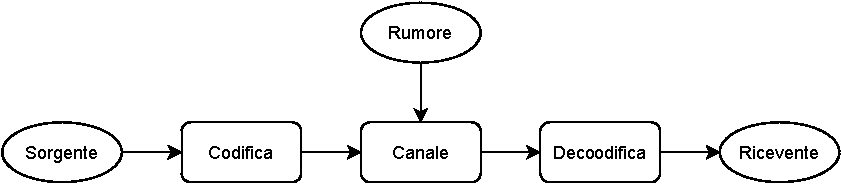
\includegraphics[width = \textwidth]{img/teo.pdf}
  \caption{Schema di un sistema generale di comunicazione tipico della teoria
    dell'informazione} 
  \label{fig:teo}
\end{figure}
Avendo:
\begin{itemize}
  \item la \textbf{sorgente} che produce segnali, dei simboli, che potrebbero
  essere continui (come la corrente), anche se noi li assumeremo come simboli di
  un alfabeto finito, avendo quindi una \textbf{sorgente discreta}
  \item i simboli, per poter essere spediti all'interno di un canale, vanno
  codificati, avendo una parte di \textbf{codifica}
  \item una volta codificati i simboli vanno nel \textbf{canale di
    trasmissione}, dove si ha del \textbf{rumore}. Tale \textit{rumore} prende
  un simbolo di quelli inseriti e lo cambia
  \item dal canale esce o il simbolo che è entrato o il simbolo modificato dal
  rumore e, tipicamente, non è immediatamente utilizzabile ma deve passare per
  una fase di \textbf{decodifica}
  \item il simbolo decodificato arriva al \textbf{destinatario}
\end{itemize}
Si hanno
alcune assunzioni sulla sorgente:
\begin{itemize}
  \item è \textbf{discreta}, i simboli emessi appartengono ad un alfabeto
  finito. Normalmente tali simboli sono $S=\{s_1, s_2,\ldots,s_q\}$
  \item i simboli vengono emessi uno alla volta ad ogni \textbf{colpo di
    clock}. Non si ha mai che in un colpo di clock non escano simboli o che ne
  escano più di uno solo 
  \item la sorgente è \textbf{senza memoria (\textit{memoryless})}, avendo che
  i simboli già usciti non influenzano per nulla il simbolo che sta per
  uscire. Ogni simbolo che esce non tiene conto del passato
  \item è \textbf{probabilistica e randomizzata}. Si ha quindi che i simboli
  $S=\{s_1, s_2,\ldots,s_q\}$ escono con le probabilità
  $(p_1,p_2,\ldots,p_q)$. Deve valere che, ovviamente, che $p_i\in
  [0,1],\forall
  i=1,\ldots,q$. Si ha inoltre che le varie probabilità, nel loro insieme,
  devono formare una distribuzione di probabilità, avendo che:
  \[\sum_{i=1}^q p_i=1\]
  Potrei avere simboli con probabilità nulla di comparire ma nella pratica non
  è qualcosa di sensato. La sorgente la costruisco o da zero (e a quel punto
  un simbolo con probabilità nulla non lo metterei) o ho una sorgente che devo
  studiare (e qui potrei avere simboli con probabilità bassissime se non
  nulle, in tal caso bisognerebbe rivalutare l'assunzione dei simboli di
  quella sorgente). Possiamo quindi meglio dire che $p_i\in (0,1],\forall
  i=1,\ldots,q$.\\
  D'altro canto vedo se posso avere probabilità pari a 1 per un simbolo ma in
  tal caso avrei solo quello e non sarebbe interessante. Si ha quindi che:
  \[p_i\in (0,1),\forall i=1,\ldots,q\]
  \[\sum_{i=1}^q p_i=1\]
  \textit{Le sorgenti che emettono i simboli secondo  
    uno schema prefissato, deterministico, sono poco interessanti, avendo un
    comportamento banale}
\end{itemize}
La parte di \textit{codifica e decodifica} può essere approfondita. Nello schema
in figura \ref{fig:teo} ci si è infatti concentrati sul canale, avendo che la
codifica serve a fare in modo che il simbolo trasmesso vada bene per essere
trasmesso nel canale. La \textbf{codifica} è a sua volta suddivisa in due parti:
\begin{enumerate}
  \item \textbf{codifica di sorgente}, che ha come obiettivo rappresentare nel
  modo più efficiente e compatto i simboli emessi dalla \textit{sorgente}. Si
  vuole quindi comprimere la sequenza di simboli (messaggi) emessi dalla
  sorgente, per impegnare meno banda possibile quando andremo a spedire. Si deve
  considerare che ogni bit in un file 
  compresso è essenziale per permettere di poter recuperare il contenuto
  compresso 
  \item \textbf{codifica di canale}, che ha quasi uno scopo opposto rispetto
  alla \textit{codifica di sorgente}, infatti ha come obiettivo quello di
  contrastare il rumore e per farlo aggiunge ridondanza al messaggio (da qui il
  discorso sull'obiettivo opposto)
\end{enumerate}
Si cerca quindi di comprimere il più possibile nella prima fase, quella di
\textit{codifica di sorgente} e di ridondare il meno possibile nella seconda,
quella di \textit{codifica di segnale}.\\
Per capire meglio quanto detto diamo alcune formalità.
\begin{definizione}
  Una \textbf{codifica} è una funzione $cod$ che prende i simboli della sorgente
  $S=\{s_1, s_2,\ldots,s_q\}$ e ad ogni simbolo $s_i$ gli assegna una stringa
  formata coi caratteri di un certo alfabeto $\Gamma$, l'\textbf{alfabeto
    della codifica}. Le stringhe di $\Gamma^*$ sono tutte quelle costruite
  sull'alfabeto $\Gamma$ di lunghezza arbitraria e finita, compresa la stringa
  vuota $\varepsilon$, che posso quindi formare coi simboli di $\Gamma$. Quindi
  ad ogni $s_i\in S$ assegno un $\gamma_i\in Gamma^*$, avendo che:
  \[cod:S\to \Gamma^*\]
  
\end{definizione}
Si hanno quindi i simboli $S=\{s_1, s_2,\ldots,s_q\}$ che escono con
probabilità $(p_1,p_2,\ldots,p_q)$ e che vengono codificati con le stringhe
$\gamma_1,\gamma_2,\ldots,\gamma_q$. Le varie $gamma_i$ sono dette
\textbf{codeword}. Chiamando $l_i=|\gamma_i|$ la lunghezza 
di tali stringhe si ha che tali stringhe hanno associati i vari
$l_1,l_2,\ldots,l_q$.\\
L'obiettivo quindi della \textit{codifica di sorgente} è quello di minimizzare
la lunghezza media $L$ delle stringhe, avendo quindi una media pesata (pesata
sulle probabilità):
\[L=\sum_{i=1}^q p_i\cdot l_i\]
Tenendo conto delle probabilità, per minimizzare $L$, si deve, avendo a che fare
con termini che sono tutti $>0$ (avendo supposto che non si hanno probabilità
nulla e avendo che una codeword pari alla stringa vuota ha poco senso), fare in
modo che i termini siano tutti il più piccolo possibile. Dato che le probabilità
sono date mentre la codifica la sto costruendo, calcolando le codeword e di
conseguenza le loro lunghezze, devo fare in modo che se la probabilità è grande
la lunghezza deve essere piccola. Se invece la probabilità è piccola posso
permettermi una lunghezza più grande. Parto quindi dai simboli con probabilità
più grande e inizio a usare codeword più piccole possibili, usando via via
quelle più lunghe. \\
Un'idea simile è usata nel \textit{codice Morse} dove le
lettere meno comuni hanno le sequenze più lunghe di punti, linee e spazi (avendo
una codifica ternaria). La lettera più comune, la ``e'', ha infatti solo con un
punto, la codifica più breve mentre le meno comuni hanno sequenze multiple di
punti, linee e spazi che le separano (e gli spazi contano nella lunghezza di
queste codeword).\\
Noi non sappiamo in anticipo che messaggi verranno prodotti dalla sorgente e
quindi le codeword vanno studiate passo a passo, valutando i simboli più
probabili per associare le codeword più brevi e i meno probabili per le
codeword più lunghe.\\
Analizziamo meglio i codici, le codeword. Possono essere:
\begin{enumerate}
  \item \textit{a lunghezza fissa}, ovvero si ha che $l_1=l_2=\cdots=L_q$
  \item \textit{a lunghezza variabile}, avendo che ogni codeword può avere
  lunghezza diversa
\end{enumerate}
Ne segue quindi che il discorso di minimizzare $L$ ha senso solo in presenza di
\textit{codeword a lunghezza variabile} (potendo decidere per ogni simbolo che
codeword associare).\\
Con \textit{codeword a lunghezza fissa} avrei tutte le $l_i$ uguali e quindi
avrei, avendo $l_i=l,\forall i$:
\[L=\sum_{i=1}^q p_i\cdot l_i \sum_{i=1}^q p_i\cdot l =l\cdot\sum_{i=1}^q
  p_i=l\cdot 1 = l\]
avendo, come facilmente intuibile, che la lunghezza media è la lunghezza fissa
stessa. Si hanno codifiche a lunghezza fissa, come banalmente numeri a 64bit
etc$\ldots$\\
Usando codifiche a lunghezza fissa si hanno anche esempi interessanti come
quello del \textit{codice pesato}, detto \textbf{codice pesato 01247}. Il nome
deriva dal fatto che si possono codificare le cifre da 0 a 9 (da 1 a 9 con poi
lo 0 dopo il 9) sotto forma di stringhe di 5 bit usando i pesi 0,1,2,4,7
associati a ciascun bit. Vediamo la tabella con la codifica di questo codice:
\begin{table}[H]
  \centering
  \begin{tabular}{c|ccccc} 
    & 0 & 1 & 2 & 4 & 7 \\
    \hline
    1 & 1 & 1 & 0 & 0 & 0 \\
    2 & 1 & 0 & 1 & 0 & 0 \\
    3 & 0 & 1 & 1 & 0 & 0 \\
    4 & 1 & 0 & 0 & 1 & 0 \\
    5 & 0 & 1 & 0 & 1 & 0 \\
    6 & 0 & 0 & 1 & 1 & 0 \\
    7 & 1 & 0 & 0 & 0 & 1 \\
    8 & 0 & 1 & 0 & 0 & 1 \\
    9 & 0 & 0 & 1 & 0 & 1 \\
    0 & 0 & 0 & 0 & 1 & 1
  \end{tabular}
\end{table}
Si nota che ogni codeword ha sempre 3 bit pari a 0 e due bit pari a 1, avendo un
\textbf{codice 2-su-5}. Banalmente i pesi si associano ai numeri 0,1,2,4,7 in
modo tale che essi, sommati, formino il numero voluto (ad esempio per 1 avrò i
pesi su 0 e 1, per 9 su 2 e 7 etc$\ldots$). L'unico caso è il caso dello 0, che
non può essere ottenuto come somma di due pesi (spesso si hanno nei codici casi
speciali da gestire a parte). Per lo 0 viene quindi presa una codeword non usata
per altri numeri e quindi l'unica scelta possibile è avere i pesi su 4 e 7
(visto che farebbe 11).\\
Su un totale ci 5 bit, avendo due bit a 1 e tre bit a 0, posso avere un numero
di codeword pari a:
\[n={{5}\choose{2}}=10\]
avendo che i 5 bit sono associati ai 5 elementi dove 1 segnala che ``sto usando
quel peso'', prendendo quindi i sottoinsiemi di due elementi a partire da un
insieme di cinque elementi, ovvero ``in quanti modi posso formare sottoinsiemi
che contengono due elementi a partire da un insieme di cinque elementi'' o detto
altrimenti ``quanti sono i modi in cui posso disporre due uni all'interno di una
stringa di cardinalità cinque''.\\
In un linguaggio di programmazione privo di una struttura dati dedicata posso
simulare un insieme di questo tipo tramite un vettore di bit (con 1 se
l'elemento associato all'indice c'è).\\
\textit{Il codice a barre è detto \textbf{codice 39} ed è un \textbf{codice
    3-su-9}}. \\
In merito alla \textbf{decodifica} si ha che anch'essa sarà di due tipi:
\begin{enumerate}
  \item \textbf{decodifica di canale}, vedendo e c'è stato un errore di
  trasmissione ed eventualmente correggendolo in automatico se il codice mi
  consente di farlo
  \item \textbf{ulteriore decodifica} che non è esattamente una \textit{codifica
    di sorgente} ma quanto una \textit{trasformazione}, dove le
  \textit{codeword} vengono trasformate nel formato leggibile dal
  \textbf{ricevente} 
\end{enumerate}
\section{Codici per individuare errori}
Ci concentriamo ora sulla \textit{codifica di canale} ignorando per ora la
\textit{codifica di sorgente}, avendo come obiettivo l'aggiunta di ridondanza a
simboli, che si suppongono già codificati con codeword, in modo tale che in
queste codeword, spedite nel canale dove eventualmente si possono avere
modifiche causate dal rumore, vengano eventualmente riconosciuti (ed
eventualmente corretti) errori in fase di \textit{decodifica}.\\
Qualora il ricevente con la sua decodifica si accorga che è successo qualcosa ma
non si è in grado di 
correggere quel qualcosa si hanno i cosiddetti \textbf{codici per individuare
  gli errori (\textit{error detection codes})}. Nel caso in cui il ricevente con
la sua decodifica si accorga dell'errore ci si chiede anche se può correggerlo
autonomamente senza chiedere che la sorgente spedisca nuovamente il
messaggio. Non sempre questa cosa si può fare ma quanto accade si parla di
\textbf{codici a correzione d'errore (\textit{error correction codes})}.
\begin{definizione}
  Si definisce il \textbf{controllo di parità}. \\
  Avendo una sequenza di $n$ bits in
  cui si ha $n-1$ bits, dette \textbf{cifre di messaggio} di \textbf{messaggio vero}, che chiameremo
  \textbf{\textit{msg}} e un bit che è la \textbf{cifra di controllo}, che
  chiameremo \textbf{\textit{check}}. Le cifre di messaggio si indicano con
  $\circ$ mentre la cifra di controllo con $\times$ e quindi il messaggio è del
  tipo:
  \[\circ\circ\circ\circ\cdots\circ\times\]
  avendo $n-1$ $\circ$ e u $\times$.\\
  Si ha che:
  \begin{itemize}
    \item chi spedisce ha le cifre di messaggio e deve calcolare la cifra di
    controllo
    \item chi riceve controlla che la cifra di controllo sia coerente con le
    cifre di messaggio
  \end{itemize}
  \textbf{To be continued...}
\end{definizione}
\end{document}
% LocalWords:  clock
